% !TEX root = ../main.tex
\chapter{Results \& Discussion}

\section{Determination of Extraction Conditions} % (fold)
\label{sec:determination_of_extraction_conditions}

	Preliminary experiments demonstrated, that the antibiotic compound could not be extracted with ethyl acetate.
	Only culture broth supernatant of the complex media NL~200, NL~300, NL~500 and OM produced notable inhibition zones on plate bioactivity assays.
	Moreover, the compound was not retained in any matter, when the supernatant was separated by HPLC with a common reverse-phase method.
	The compound is likely very hydrophilic, so that usual extraction and reverse-phase chromatography protocols are not applicable.
	Because of the difficulties involved in working with aqueous solvents, an extraction procedure involving organic solvents would be beneficial.
	Additionally, out of the four complex media, in which Tü2401 is able to produce the antibiotic, one with optimal properties has to be determined.

\subsection{Comparison of Production Media} % (fold)
\label{sub:comparison_of_production_media}

	To determine the optimal production medium, Tü2401 was grown in each of the NL and OM media for either four or seven days.
	The obtained medium supernatants were filtrated by using \SI{0.45}{\micro\meter} and \SI{0.2}{\micro\meter} consecutively.
	OM supernatant proved to be the easiest to filtrate, while the NL media clogged the filters after few milliliters had passed through.
	Each filtrate was subjected to the standard bioassay against \textit{Escherichia coli}~K12 to determine the antibiotic activity.
	Pictures of the assay results are displayed in Figure~\ref{fig:medium_activity}.
	
	\begin{figure}[htbp]
	\centering
		\begin{subfigure}{0.5\textwidth}
			\includegraphics[width=0.8\textwidth]{medium_activity_96}
			\caption{Four day growth period}
		\end{subfigure}%
		\begin{subfigure}{0.5\textwidth}
			\includegraphics[width=0.8\textwidth]{medium_activity_168}
			\caption{Seven day growth period}
		\end{subfigure}
		\caption[K12 Bioassay results with media supernatants]{%
			\textbf{K12 Bioassay results with media supernatants}
			\textit{Streptomyces}~sp.~Tü2401 was grown for either four (a) or seven days (b) in four different complex media.
			The filtrated medium supernatant was tested against \textit{Escherichia coli}~K12.
			Media: (Top) NL~200 (Left) NL~300 (Right) NL~500 (Bottom) OM.}
		\label{fig:medium_activity}
	\end{figure}
	
	Most samples caused notable ($\varnothing>$\SI{1}{\centi\meter}) zones of inhibition in the agar diffusion assay.
	NL~500 after seven days and OM in both cases possess the greatest activity with inhibition zones greater than \SI{1.5}{\centi\meter}.
	When cultivated in NL~300, Tü2401 seems to take longer than four days to synthesize the compound.
	NL~500 and OM supernatants were separated via an Agilent~1200 HPLC system equipped with a diode array detector (DAD) and evaporative light scattering detector (ELSD).
	A C18 column was used in combination with a 4.5~\% to 100~ \% acetonitril screening gradient (see Table~\ref{tab:method_c18_screening}).
	The chromatograms are shown in Figure~
	
	\begin{figure}[htbp]
		\centering
		\begin{subfigure}{0.8\textwidth}
			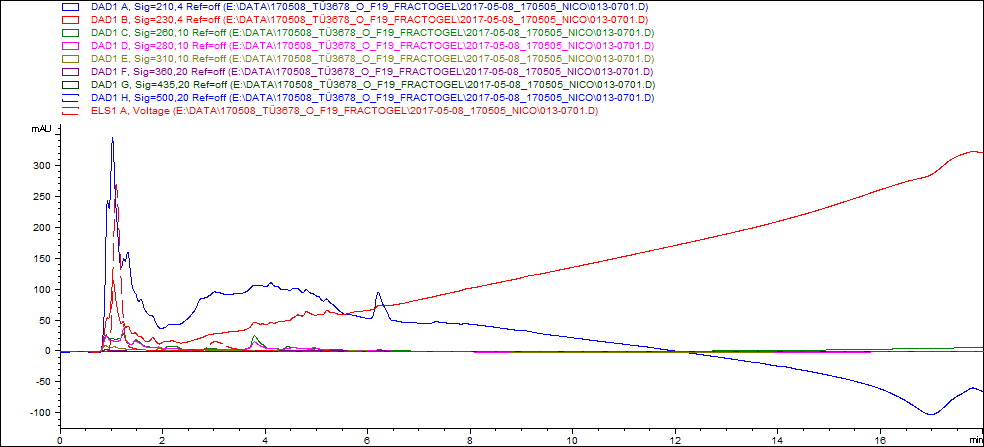
\includegraphics[width=\linewidth]{media_sup_500}
			\caption{NL 500 medium supernatant}
		\end{subfigure}
		\begin{subfigure}{0.8\textwidth}
			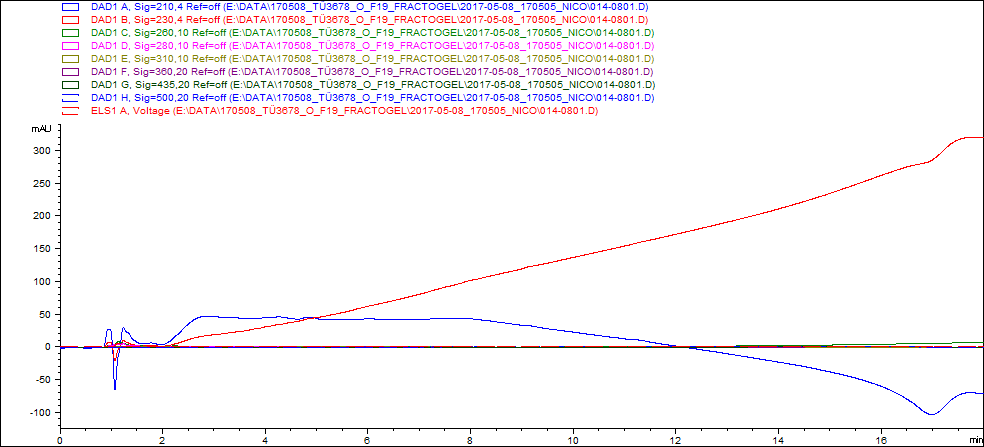
\includegraphics[width=\linewidth]{media_sup_om}
			\caption{OM medium supernatant}
		\end{subfigure}
		\caption[Chromatogram of medium supernatant screening]{%
			\textbf{Chromatogram of medium supernatant screening.}
			\SI{5}{\micro\liter} of medium supernatant were injected and separated on a C18 column.
			A screening gradient of 4.5 to 100~\% acetonitril was employed.
			UV absorption and ELSD voltage were measured.}
		\label{fig:results_medium_screen}
	\end{figure}
	
	The screening chromatograms show, that most compounds in the medium supernatants are rather hydrophilic.
	No UV absorption or ELSD voltage peaks can be observed after \SI{7}{\minute}.
	In the case of OM, only the injection peak is present.
	The OM supernatant seems to predominantly contain compounds, that can not be separated with a reverse-phase screening gradient on a C18~column.
	Since the antibiotic compound of interest showed no retention under similar conditions, the use of OM as a production medium would result in fewer impurities in the hydrophobic spectrum.
	Combined with the visible antibacterial activity of the supernatant against \textit{E. coli}~K12 after only four days and the ease of preparation and filtration, OM was chosen as the default production medium for further experiments.
	
	\subsection{Extraction experiments}
	\label{sub:extraction_experiments}
	
	Three organic solvents, which are immiscible with water, were tested for extraction of the antibiotic compound.
	Ethyl acetate, methyl acetate and ethyl formate. Additionally, the supernatant was adjusted to five different pH~values ranging from 2 to 11.
	A hydrophilic molecule is likely to contain functional groups like amines or carboxylic acids, which are charged at certain pH-ranges.
	If the compound does too, the isoelectric point could passed by pH adjustment.
	Through reduced charge, the water-solubility could be lowered, enabling the extraction with an organic solvent.
	
	OM medium supernatant was divided into three groups of five aliquots.
	The pH of each aliquot was adjusted to either 2, 5, 7, 9 or 11.
	Each group was then extracted with either ethyl acetate, methyl acetate or ethyl formate.
	Both phases were separated and tested for bioactivity against \coli. 
	
	\begin{figure}[htbp]
		\centering
		\begin{subfigure}{\textwidth}
			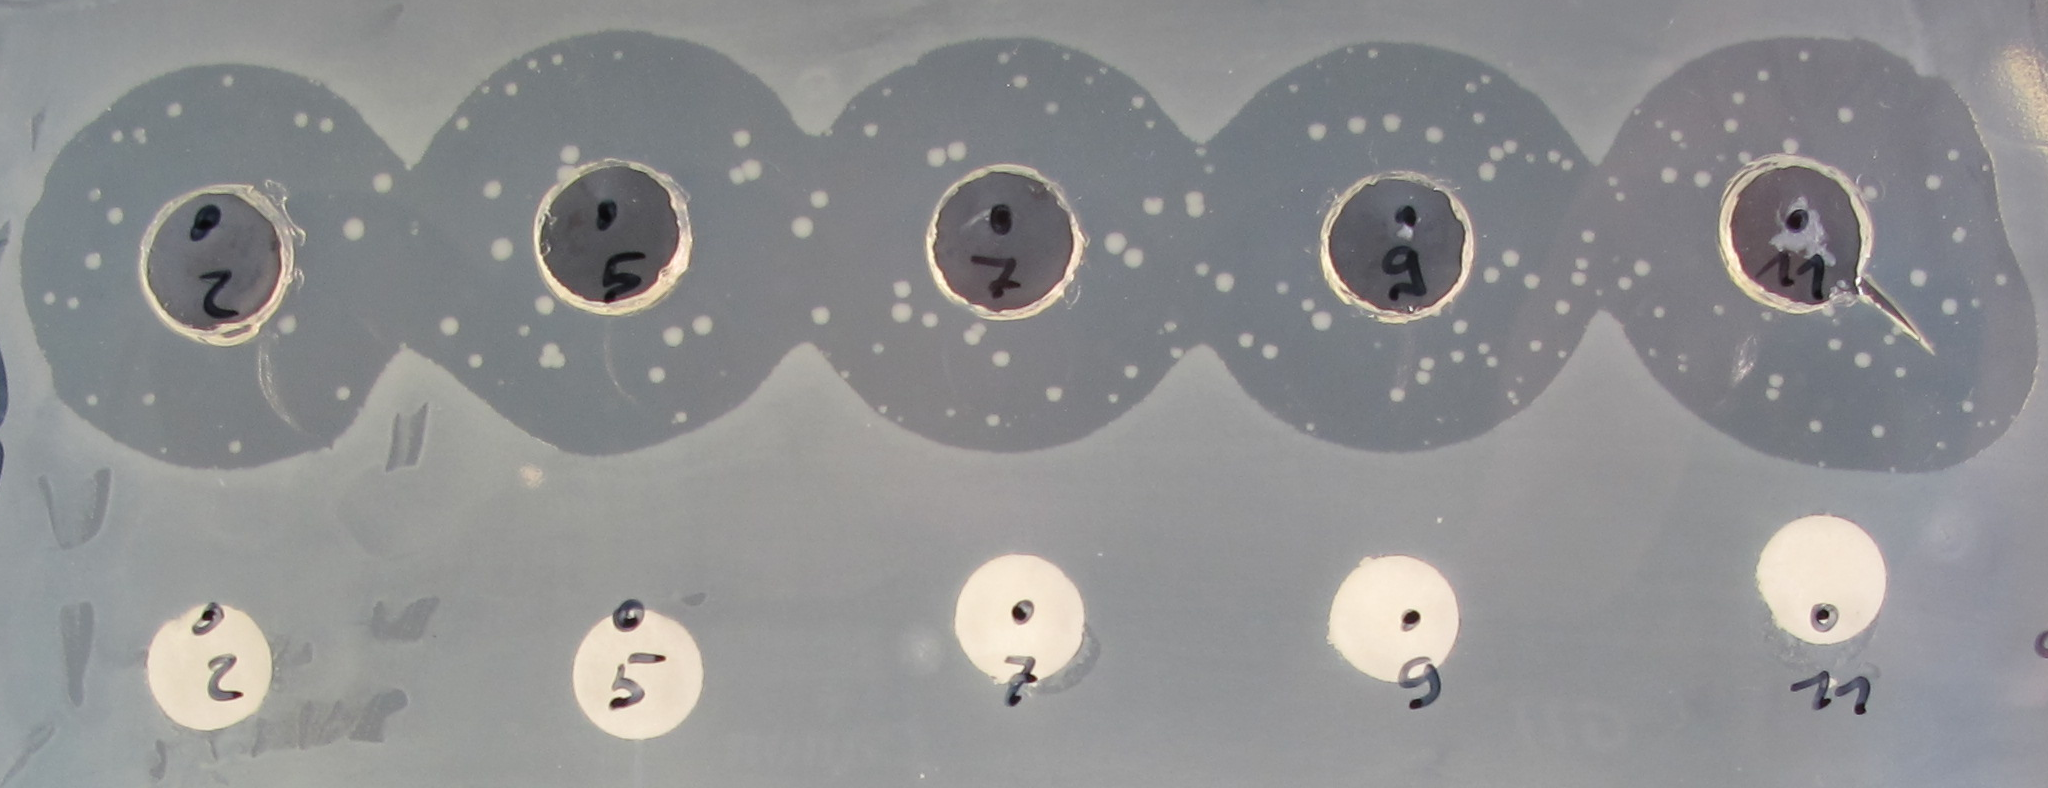
\includegraphics[width=\linewidth]{medium_ph_etac}
			\caption{Ethyl acetate}
		\end{subfigure}
		\begin{subfigure}{\textwidth}
			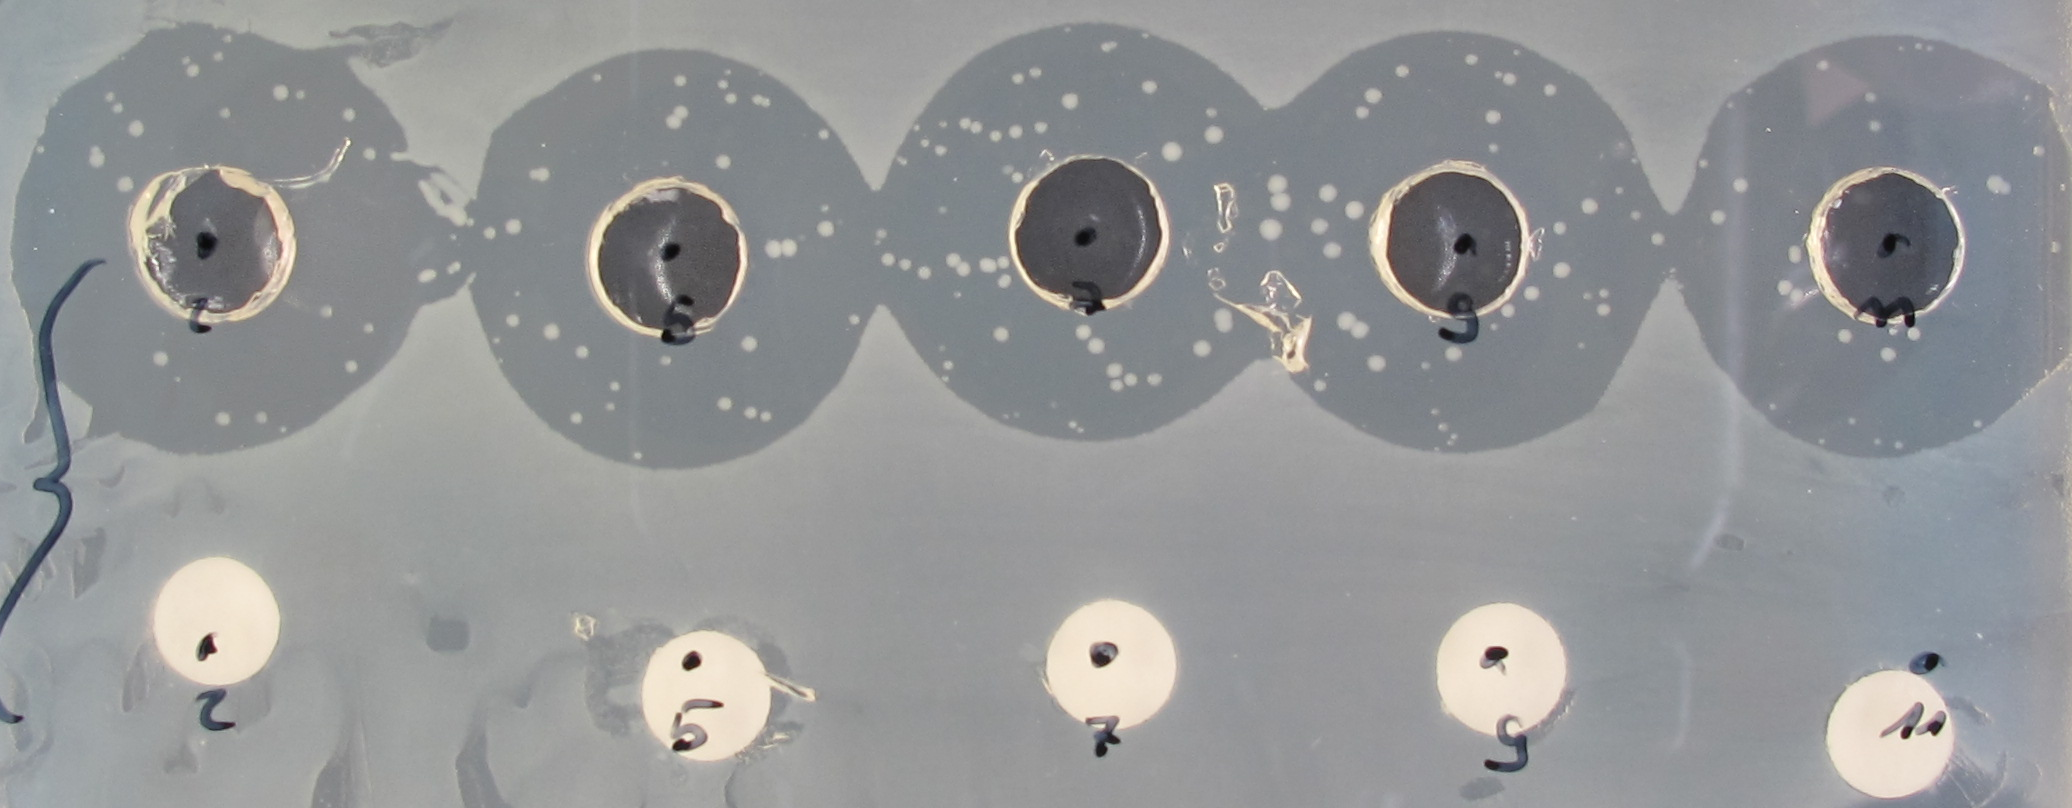
\includegraphics[width=\linewidth]{medium_ph_meac}
			\caption{Methyl acetate}
		\end{subfigure}
		\begin{subfigure}{\textwidth}
			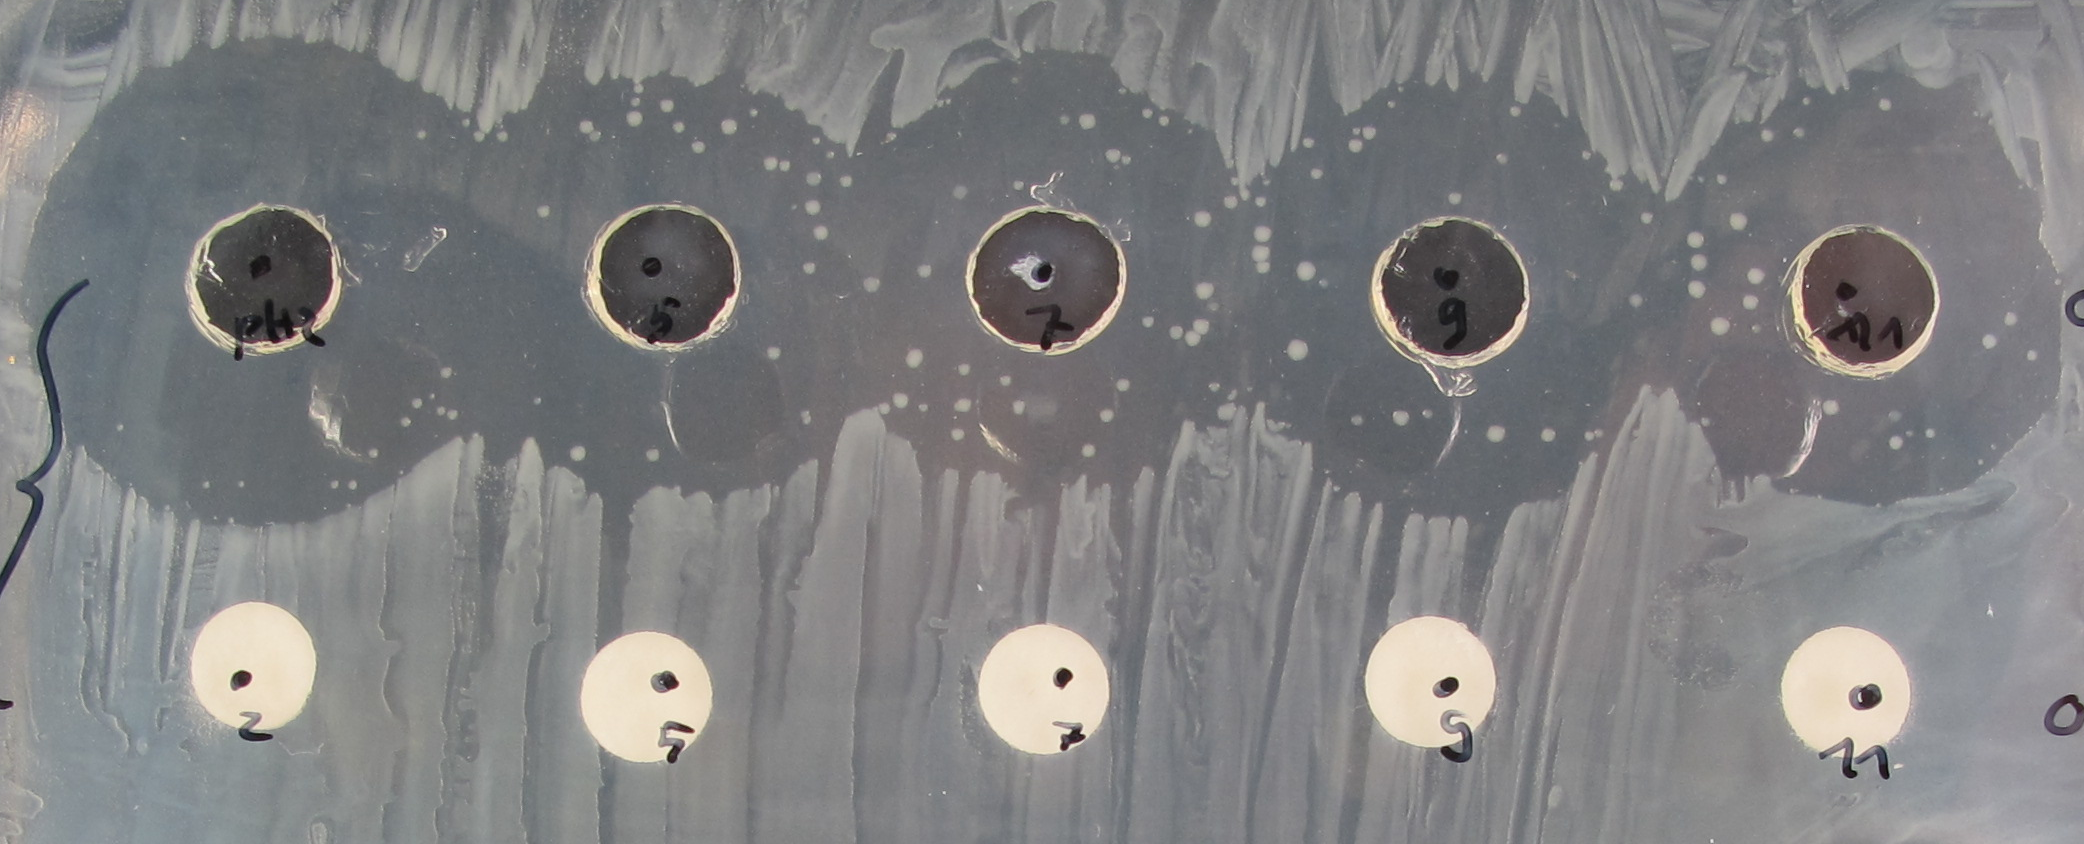
\includegraphics[width=\linewidth]{medium_ph_etform}
			\caption{Ethyl formate}
		\end{subfigure}
		\caption[Bioassay results of different OM medium extracts against \coli]{%
			\textbf{Bioassay results of different OM medium extracts against \coli}
			Filtered supernatant of OM cultures of \tue were extracted with either (a) ethyl acetate, (b) methyl acetate or (c) ethyl formate.
			Sample-pH was adjusted prior to either 2, 5, 7, 9 or 11 (left to right).
			Both phases were tested seperately.
			Upper row consists of \SI{50}{\micro\liter} aqueous phase pipetted directly into wells.
			Lower row consists of \SI{50}{\micro\liter} organic phase pipetted onto a sterile filter plate and placed on the agar.}
		\label{fig:results_extraction_bioassay}
	\end{figure}
	
	%either zwitterionic -> pH ranges too large
	%many polar, but uncharged groups
	%Chromatogramme von beiden Fraktionen
	%Wieviel konnte durch ausschütteln entfernt werden?
	
% section determination_of_extraction_conditions (end)

\section{Chromatographic Separation} % (fold)
\label{sec:results_chromatographic_separation}

    \subsection{Reverse-Phase HPLC} % (fold)
    \label{sub:results_reverse_phase_hplc}

    % subsection reverse_phase_hplc (end)

    \subsection{Hydrophilic Interaction Liquid Chromatography} % (fold)
    \label{sub:results_hydrophilic_interaction_chromatography}
    
	\begin{itemize}
		\item Short reiteration of HILIC
		\item Characteristics of NH2 column
		\item Characteristics of ZIC-HILIC column
	\end{itemize}

	The \luna by Phenomenex features a silica matrix modified with 3-aminopropyl groups.
	The used model had a particle size of \SI{3.5}{\micro\meter} and a pore size of 100~\AA.
	The dimensions were $4.6\times250$~mm.
    
	    \subsubsection{Luna NH\textsubscript{2} Column}
	    
	    Separation via the \luna column was performed with an isocratic method (see \ref{tab:method_nh2_standard}).
	    The mobile phase consisted of 80~\% acetonitrile and 20~\% water at a flow of \SI{2.0}{\milli\liter\per\minute}.
	    Both solvents contained 0.1~\% formic acid as a modifier.
	    \SI{50}{\micro\liter} of filtrated reverse extract at pH~11 were injected and fractions collected every minute.
	    The fractions were subjected to the standard agar-diffusion bioassay against \coli.
	    The chromatogram is shown in 
	    
	    % Bild im Anhang anfügen
	    
	    With this method, the water-soluble compound could be separated from the injection peak.
	    Fractions 5, 6 and 7 produced noticeable zones of inhibition, correlating to elution between 4 and 7~min.
	    With the injection peak eluting at 1.5~min, a relative retention of 2.5 to 5.5 min could be achieved.
	    The majority seems to have eluted between 3.5 and 5.5~min, since the inhibition zones of fractions 6 and 7 were the largest with a diameter of \SI{1.7}{\centi\meter}.
	    Fraction 5 only produced a diameter of \SI{1.2}{\centi\meter}.
	    In the UV-chromatogram, two baseline-separated peaks with distinct spectra were detected in the timeframe correlated to bioactivity.
	    The first was detected at 5~min, the second at 6~min. The UV-spectra  indicate that two bioactive compounds with similar retention times have eluted right between the fraction collector timeframes.
	    A single compound should have resulted in the detection of a rather broad peak with long fronting.
	    However, if the compound does not possess a UV-chromophore, an additional method of detection is needed.

		An evaporative light scattering detector (ELSD) can be used to detect analytes without chromophores, as long as they are less volatile than the solvent.\autocite{Mathews2004,Righezza1988,Mourey1984,Charlesworth1978}
		The detector can be coupled to a standard HPLC system and provides additional analytical data.
		To eliminate elution differences between different systems, both the ELSD and the fraction collector were attached to the same system behind the UV-detector.
		Since ELS-detection is inherently destructive, a splitter was used to divide the flow. One fifth was directed to the ELSD, the rest to the fraction collector.
		With both 
	    
		% Retention ähnlich wenn pH 11 oder nicht eingestellt (ph8)
		% Könnte bedeuten, dass bei beiden Werten gleich geladen wenn ionenaustausch / adsorption dominierende Kraft
		% Schlechte selektivität durch Sample mit wasser
	    
    % subsection hydrophilic_interaction_chromatography (end)

    \subsection{Ion Exchange Chromatography} % (fold)
    \label{sub:results_ion_exchange_chromatography}

	Water-soluble compounds contain polar functional groups, some of which at certain pH ranges can even be charged.
	A \pka value comparison of natural products in the Antibase2008 database revealed, that the majority of entries might be charged at pH~2--11.\autocite{Mansson2010}
	44~\% contained an acidic functionality, 17~\% a basic one, and 9~\% both.
	It is likely, that the hydrophilic antibacterial compound also contains basic or acidic functional groups such as amino- or carboxyl-groups.
	The presence of charged functionalities in a molecule can be utilized for separation via ion-exchange chromatography (IEC).
	
	%Nutzungsbeispiele für IEC

	Since as of now, not much is known about the water-soluble antibacterial compound, an explorative IEC method similar to the approach of M{\aa}nsson~\textit{et al.} was devised.\autocite{Mansson2010}
	Two ion-exchange resins with orthogonal selective properties were employed to test if the compound contains acidic or basic functionalities.
	Both feature "strong" ion exchange groups, which retain their charge over a broad pH-range and are immobilized on a divinylbenzene matrix.
	The strong cation exchanger (SCX), Dowex 50WX4, contains negatively charged sulfonic acids, while the strong anion exchanger (SAX), Diaion SA11A, contains positively charged quarternary ammonium groups.
	The sample would be adjusted to an extreme pH such as 2 or 11, where most ionizable groups should be charged, and loaded onto the column.
	Uncharged contaminants were washed away with a buffer at the sample pH and one with pH~7.
	The elution buffer had the opposite pH of the sample pH, supposedly removing the charge and washing the compound off the column.
	In case of the SAX this means that the sample was adjusted to pH~11, where acidic functionalities such as carboxyl-groups are likely negatively charged.
	At pH~7 the charge should still be retained, therefore removing impurities by washing with pH~7 and 11.
	At pH~2 however, a carboxylic acid is likely protonated.
	The loss of charge greatly reduces the affinity to the SAX and the compound should be eluted with the buffer.
	For the SCX the same principle applies, but with the pH ranges switched to allow for retention and elution of basic compounds.
	
	\SI{1}{\milli\liter} of filtrated culture broth supernatant was adjusted with \ch{NaOH} and \ch{HCl} to the appropriate pH and used as the sample for this experiment.
	The detailed method descriptions are found in section~\ref{sub:ion_exchange_chromatography}.
	All loading, washing and elution fractions were collected, concentrated and subjected to the standard bioassay against \coli.
	
	The assay plate belonging to the SAX fractions revealed bioactivity to be present in the first three out of five elution fractions.
	The loading and washing fractions were inactive.
	The the water-soluble compound is able to form an ionic bond with sulfonic acid at pH~11 and pH~7, which is broken at pH~2.
	This indicates the presence of one or more functional groups with a \pka$<7$, which are most likely carboxyl groups.
	As such, the compound might contain organic acid moieties.
	
	The tested SCX fractions exhibited no visible bioactivity at all.
	This could be due to an exceptionally strong bond of the compound to the cationic resin, which is still present at pH~11.
	A strongly basic alkaloid or amine with a \pka$>11$ for the protonated form would not have been eluted at the used pH.
	The only other possibility would be a reaction with the SCX matrix, either deactivating the compound or binding it irreversibly.
	Degradation at extreme pH values is unlikely, since the same buffers were used for the SAX column.
	Additionaly, the compound has been observed to be exceptionally stable at pH~2--11 in water.
	Samples stored at \SI{8}{\celsius} and various pH levels have been tested for bioactivity several months after generation and displayed no noticeable loss in activity.
	
	
	
    % subsection ion_exchange_chromatography (end)

\subsection{Thin-Layer Chromatography} % (fold)
\label{sub:results_thin_layer_chromatography}
    
    %Antibiotische Zucker?
    
    A classic method for separation of sugars is thin-layer chromatography (TLC).
    %

    % subsection thin_layer_chromatography (end)
    
    \subsection{Gel-filtration} % (fold)
    \label{sub:results_gel_filtration}

% section chromatographic_separation (end)

\section{Dereplication} % (fold)
\label{sec:dereplication}

    \subsection{HPLC Mass Spectrometry} % (fold)
    \label{sub:hplc_mass_spectrometry}

    % subsection hplc_mass_spectrometry (end)

    \subsection{Trimethylsilane Derivatization and Gas Chromatography} % (fold)
    \label{sub:trimethylsilane_derivatization_and_gas_chromatography_results}

    % subsection trimethylsilane_derivatization_and_gas_chromatography (end)
    
    %mögliche Detektion falls zucker:

% section dereplication (end)

\section{Antibacterial Activity Spectrum} % (fold)
\label{sec:antibacterial_activity_spectrum}


    \subsection{Activity against \textit{Escherichia coli} K12} % (fold)
    \label{sub:activity_against_e_coli}

    % subsection activity_against_e_coli (end)

    \subsection{Activity against \textit{Bacillus subtilis} 168} % (fold)
    \label{sub:activity_against_b_subtilis}

    % subsection activity_against_b_subtilis (end)

    \subsection{Extraction of yorB-inducing Compound} % (fold)
    \label{sub:extraction_of_yorb_inducing_compound}

    Tü2401 displayed positive results in the yorB-Assay \todo{Referenz einsetzen} when grown on ISP2 plates \todo{Referenz einsetzen}.
    However, all previously generated samples from liquid cultures only showed antibacterial activity.
    %%%%%%%%%%%%%%
    %Einsetzen:
    %%%%%%%%%%%%%%
    % Absatz über Differenzierung von Streptomyceten
    % Einfluss auf Sekundärmetabolismus
    % Überleitung zu Schlussfolgerung: Evtl zweiter Compound nur auf agar produziert
    %%%%%%%%%%%%%%%
    Three cultivation strategies were developed to induce production of the putative compound 2 (PC2):

    \begin{enumerate}
        \item
	        Standing cultures could allow the formation of aerial mycelium at the medium surface.
	        Thus, enabling the synthesis of PC2 and allowing extraction of the liquid medium.
	        Two \SI{500}{\milli\liter} flasks were each filled with \SI{100}{\milli\liter} of liquid ISP2 medium and inoculated with \SI{1}{\milli\liter} of a one-week old NL~410 shake culture.
	        One flask was sealed with an ordinary aluminium cap (AC), the other one with an air-permeable foam cap (FC).
	        Both flasks were cultivated for four days, before the medium was centrifuged and the supernatant filtrated.
	        \SI{50}{\milli\liter} aliquots of each flask were extracted with either BuOH or EtAc, and both phases were collected seperately.
	        The organic phases were dried at \SI{40}{\celsius} and solved in \SI{1}{\milli\liter} MeOH.
	        Both phases of each flask were subjected to the yorB-Assay.
        \item
	        ISP2 agar plates were previously known to enable synthesis of PC2 and could be extracted with prior breakup.
	        Ten round ISP2 agar plates were inoculated with \SI{100}{\micro\liter} of a one-week old NL~410 shake culture and incubated for four days.
	        One half of the plates was extracted with BuOH, the other half was extracted with EtAc.
        \item
	        ISP2 agar plates could also be prepared with low-melting-point agarose (LMPA).
	        This would allow melting of the plates at lower temperatures.
	        Thus, allowing for easier extraction with reduced risk of thermal decomposition during the process.
	        Six ISP2 LMPA agar plates were inoculated with \SI{100}{\micro\liter} of a week-old NL~410 shake culture and incubated for four days.
	        The plates were then melted at \SI{70}{\celsius} and extracted with BuOH and EtAc.
    \end{enumerate}

    All generated extracts and their respective aqueous phases were tested for bioactivity.
    The standard bioassay was used to determine the antibiotic activity against \textit{E. coli} K12 and \textit{B. subtilis} 168, while the yorB-Assay was used to test for the mode of action.
    Additonally, agar stamps of grown ISP2 and ISP2 LMPA plates were tested in the yorB-Assay.
    A summary of the results is shown in .

    \begin{table}[htbp]
        \caption[Bioassay results from agar-plate and standing culture extraction]{%
        	\textbf{Bioassay results from agar-plate and standing culture extraction}.
	        Samples were screened for antibiotic activity against \textit{E. coli} K12 and \textit{B. subtilis} 168 and for promotor induction in the yorB-Assay.
	        Samples from standing cultures with foam cap (FC) or aluminium cap (AC), ISP2 agar plates (ISP2) and ISP2 agar plates with low-melting-point agarose (LMPA).
	        Samples were extracted with butanol (BuOH) or ethyl acetate (EtAc) and tested alongside their respective aqueous phases (aq.).\\
	        \emph{Legend}: \textbf{-} No activity; \textbf{+~/~++~/~+++} antibiotic activity with inhibition zone of 1~/~1.0-1.5~/~>1.5~cm; \textbf{n.e.} result non-evaluable}
        \label{tab:yorB_assay_results}
        \centering
        \begin{tabularx}{\textwidth}{>{\hsize=1.4\hsize}X>{\hsize=.9\hsize}X>{\hsize=.9\hsize}X>{\hsize=.9\hsize}X>{\hsize=.9\hsize}X}
            \toprule
            & \multicolumn{3}{c}{Antibacterial} & positive \\
            \cline{2-4}
            \textbf{Sample} & \textbf{\textit{E. coli}}     & \textbf{\textit{B. subtilis}}  & \textbf{yorB}  & \textbf{yorB}    \\
            \midrule
            FC BuOH         & -     & -     & -     & -    \\
            FC BuOH aq.     & -     & -     & -     & -    \\
            FC EtAc         & -     & +++   & ++    & -    \\
            FC EtAc aq.     & -     & -     & -     & -    \\
            AC BuOH         & -     & -     & -     & -    \\
            AC BuOH aq.     & -     & -     & -     & -    \\
            AC EtAc         & -     & -     & +     & -    \\
            AC EtAc aq.     & -     & -     & -     & -    \\
            \midrule
            ISP2 BuOH       & -     & n.e.  & +++   & -    \\
            ISP2 BuOH aq.   & -     & +     & -     & -    \\
            ISP2 EtAc       & -     & ++    & -     & -    \\
            ISP2 EtAc aq.   & +     & n.e.  & -     & +    \\
            ISP2 plaque     &       &       & ++    & ++   \\
            \midrule
            LMPA BuOH       & +     & n.e.  & +++   & -    \\
            LMPA BuOH aq.   & -     & n.e.  & -     & -    \\
            LMPA EtAc       & -     & n.e.  & +++   & -    \\
            LMPA EtAc aq.   & -     & n.e.  & -     & -    \\
            LMPA plaque     &       &       & -     & -    \\
            \bottomrule
        \end{tabularx}
    \end{table}
    % subsection extraction_of_yorb_inducing_compound (end)

% section antibacterial_activity_spectrum (end)

\section{Bioinformatic Analysis} % (fold)
\label{sec:species_antismash}

    \subsection{Phylogeny of Strain Tü2401} % (fold)
    \label{sub:phylogeny_of_strain_tue2401}

	\begin{figure}[htbp]
		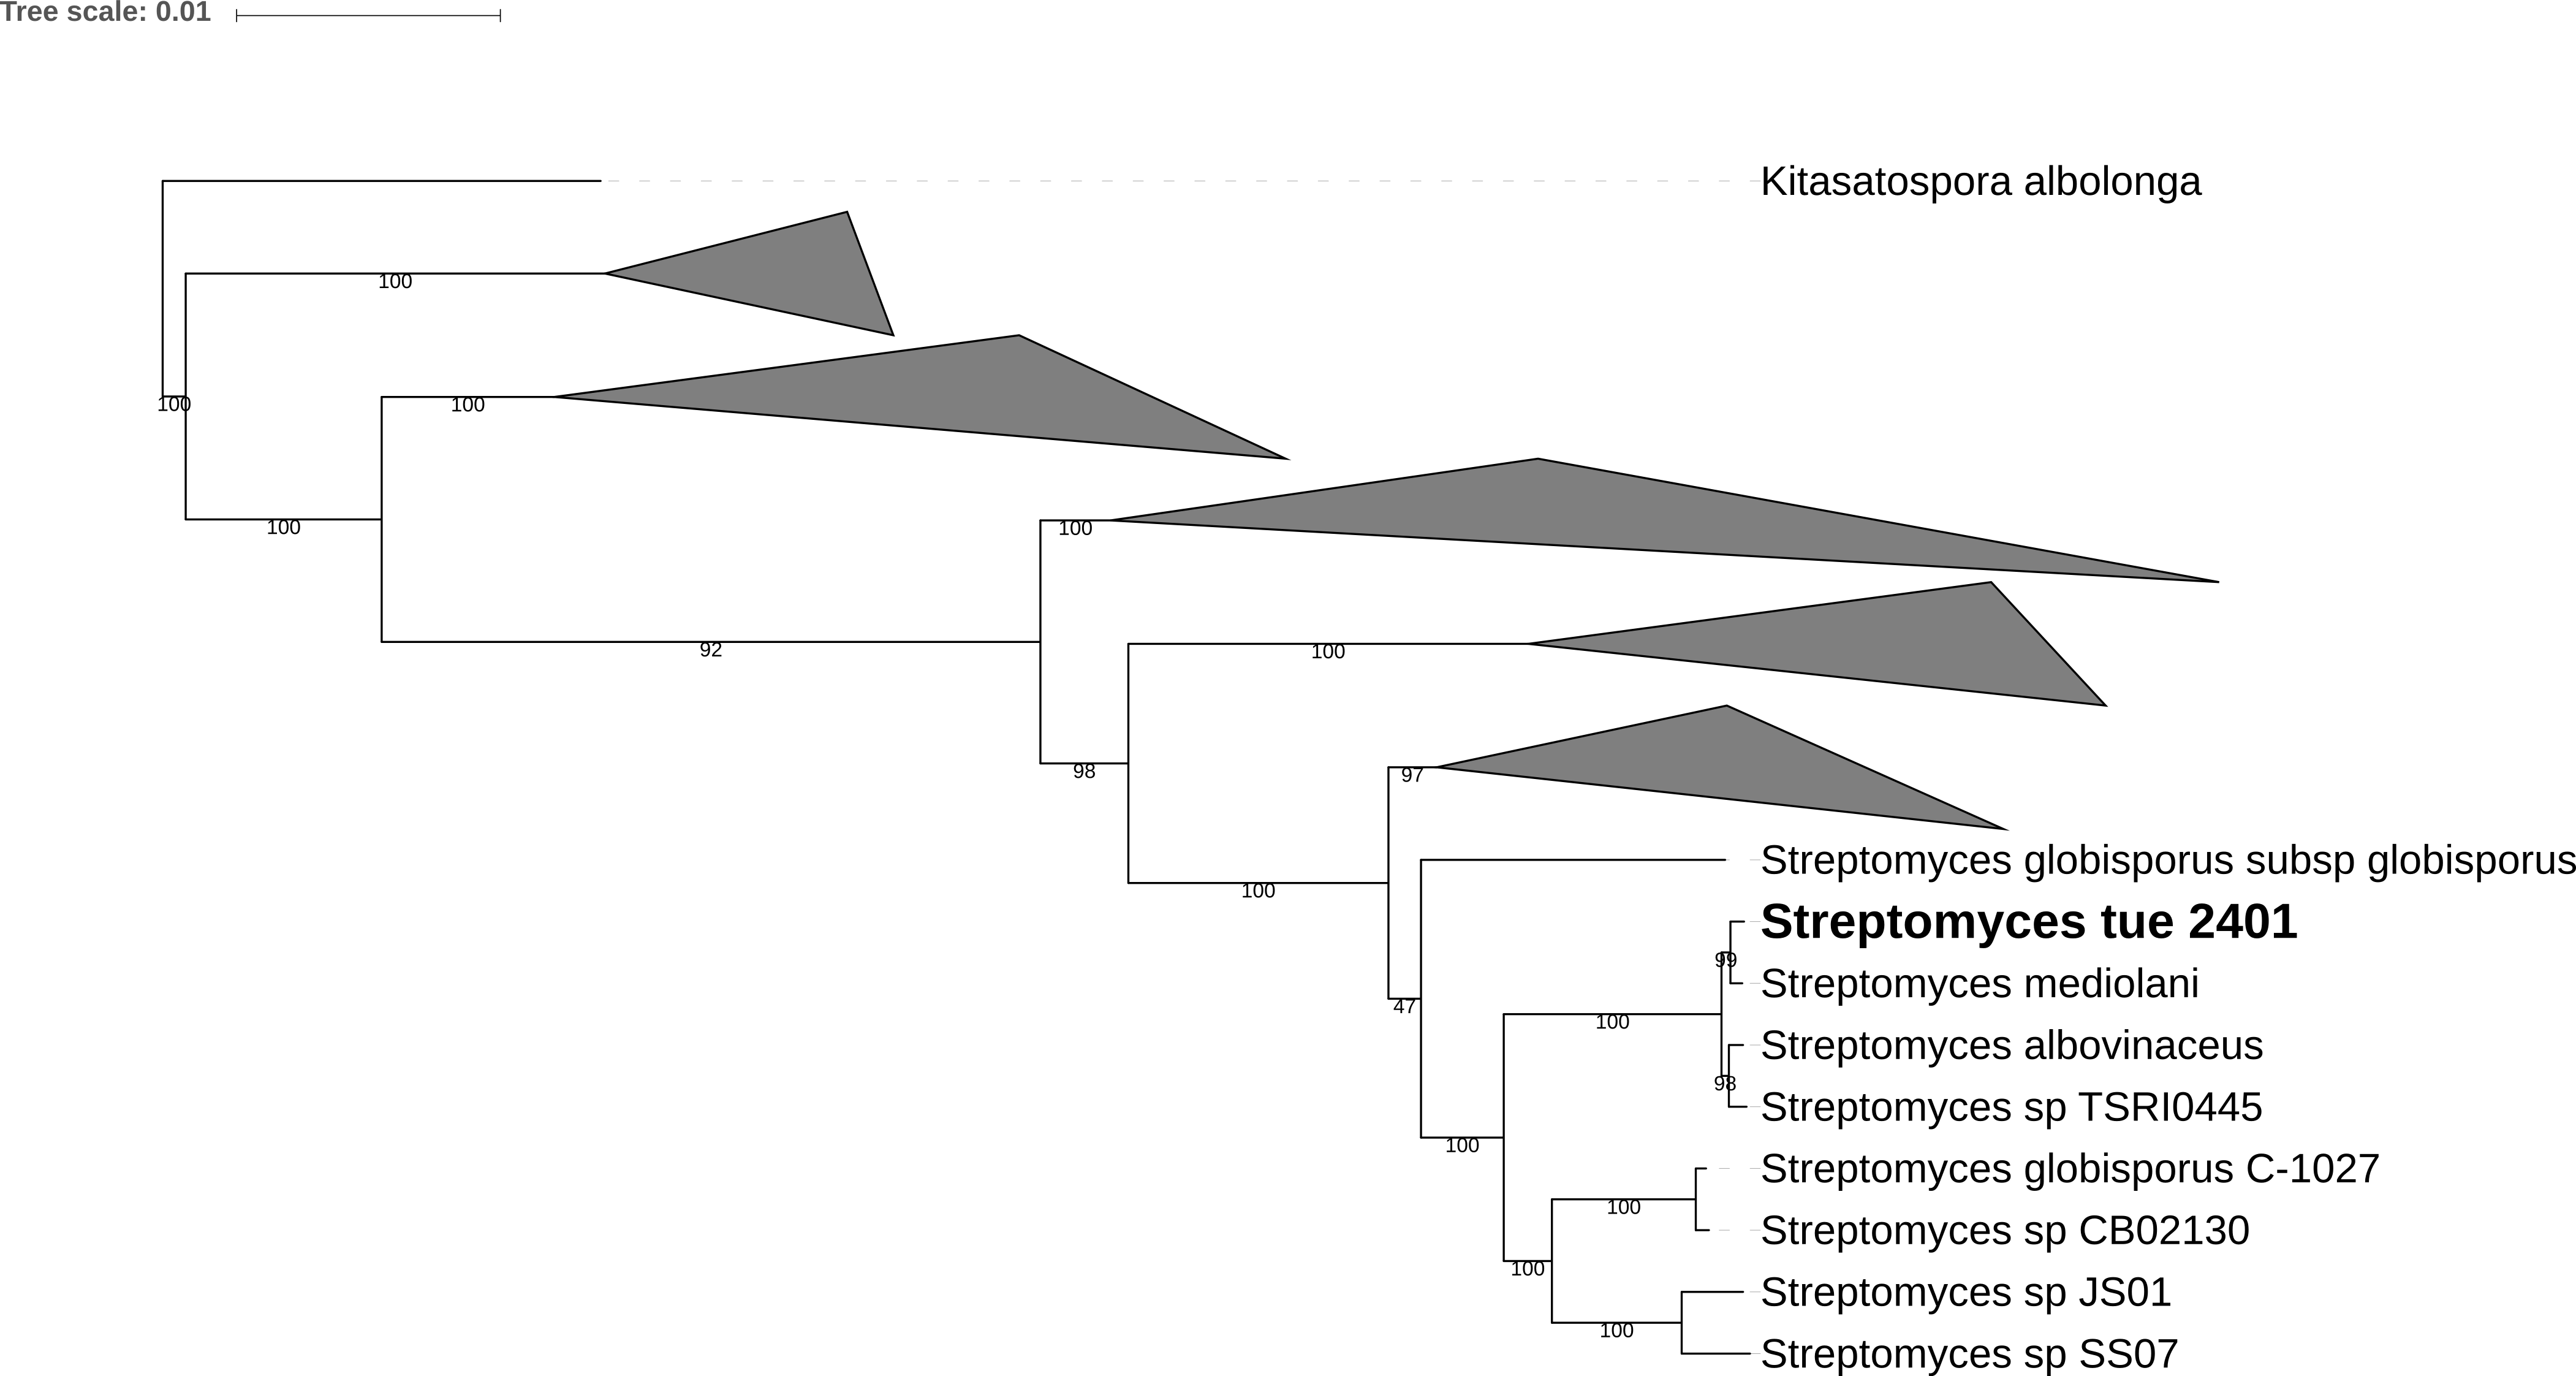
\includegraphics[width=\textwidth]{tu2401_tree}
		\caption[Maximum likelihood tree of \emph{Streptomyces} sp. Tü2401.]{%
			\textbf{Maximum likelihood tree of \emph{Streptomyces} sp. Tü2401.}
			The tree was constructed using a multiple-sequence alignment of 50 single-copy genes across 50 \textit{Streptomyces} reference genomes.
			The node belonging to \textit{Streptomyces}~sp.~Tü2401 is highlighted with bold text.
			Only the nine most closely related nodes and the outgroup are shown.
			Dark triangles represented hidden, collapsed nodes.}
		\label{fig:phylo_tree} 
	\end{figure}

    % subsection phylogeny_of_strain_tü2401 (end)

    \subsection{AntiSMASH Cluster Identification} % (fold)
    \label{sub:antismash_cluster_identification}

	 One cluster was detected on contig four and identified as a Type1-PKS-NRPS hybrid.
	 It shows a 95~\% cluster identity to the C-1027 biosynthetic gene cluster from \textit{Streptomyces} globisporus C-1027 (MiBiG accession no. BGC0000965). Additionally, three homologous subclusters with 100~\% identity were identified, which are associated with the synthesis of C-1027, Neocarzinostatin and Maduropeptin enediynes (see Figure \ref{fig:cluster_search}).
	 The presence of this cluster could indicate, that the strain Tü2401 is capable of producing a compound similar to enediyne antibiotics. 
	 
	 Enediyne natural products are a class of cytotoxic bacterial compounds, which cause extensive DNA-damage.\autocite{Liang2010,Gredicak2007,AdrianL.Smith*1996,Nicolaou1993}
	 11 different enediyne natural products are known, all of which feature either a bicyclo[7.3.0]dodecadienediyne core inside a nine-membered ring or a bicyclo[7.3.1]tridecadiynene core inside a ten-membered ring (Figure \ref{fig:enediyne_comparison}).
	 The 9-membered family includes neocarzinostatin, C-1027 and and maduropeptin.
	 The 10-membered family includes calicheamicin $\gamma_{1}^{I}$, esperamicin A\textsubscript{1} and dynemicin A.\autocite{Liang2010}
	 Enediynes are potent cytotoxic agents because of their ability to induce DNA double-strand breaks.\autocite{Shen2015}
	 Electronic rearrangement of the carbocycle produces a benzenoid diradical, which abstracts hydrogen atoms from the DNA-backbone.
	 The consulting radicals cause interstrand crosslinks or react with molecular oxygen.	 
	 \begin{figure}[htbp]
	 	\centering
	 	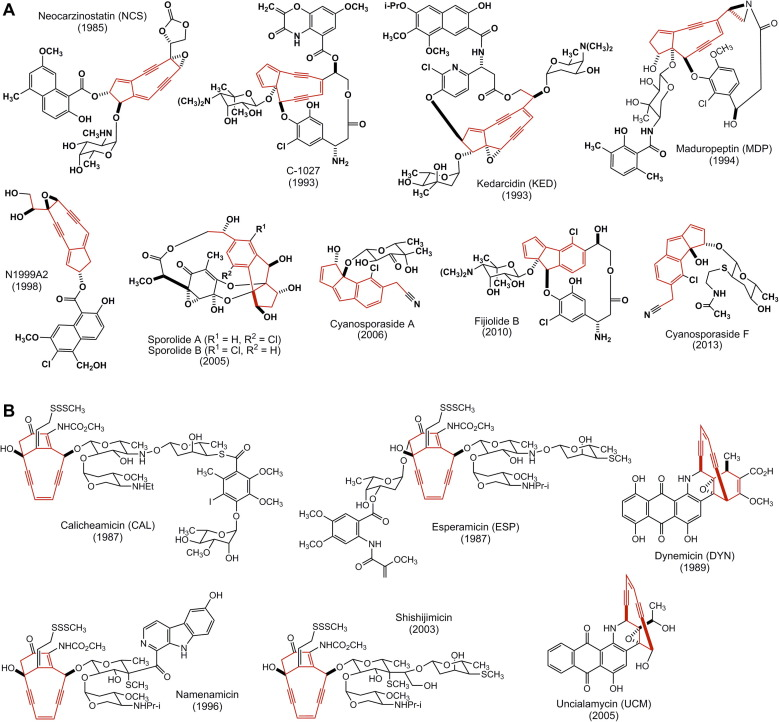
\includegraphics[width=0.9\textwidth]{enediyne_overview}
	 	\caption[Structures of known enediyne natural products]{%
	 		\textbf{Structures of known enediyne natural products.}
	 		Enediyne cores are highlighted in red.
	 		(A) Compounds with nine-membered rings.
	 		(B) Compounds with ten-membered rings.
	 		The year of structure confirmation is displayed in parentheses.
	 		The sporolides, cyanosporolids and fijiolides do not contain an endiyene core, but are proposed to be derived from enediyne precursors.
	 		Reprinted from Shen \textit{et al.} (2015) Copyright 2014 Elsevier Ltd.}
	 	\label{fig:enediyne_comparison}
	 \end{figure}
	 While the ten-membered enediyne compounds were isolated as free-standing chromophores, most of the compounds in the nine-membered family were isolated in conjunction with a protective apoprotein.\autocite{Liang2010}
	 The nine-membered chromophore of C-1027, which was isolated from \textit{Streptomyces} globisporus C-1027, is bound noncovalently to an 110 amino acid apoprotein.\autocite{AdrianL.Smith*1996,Minami1993,Yoshida1993,Otani1993,Sugiura1993,Matsumoto1993,Otani1991,Otani1988a,Matsumoto1993a}
	 The isolated chromophore has been shown to be very unstable, whereas the holo C-1027 did not lose activity under the same conditions.\autocite{Matsumoto1993,Sugiura1993,Otani1991}
	 The apoprotein binds specifically to the C-1027 chromophore, supposedly by hydrophic pocket, which binds the benzoxazine side chain.\autocite{Okuno1994,Matsumoto1993}
	 The enediyne antibiotics neocarzinostatin and maduropeptin, which were also isolated from actinomycetes, feature highly specific and protective apoproteins as well.\autocite{AdrianL.Smith*1996}.
	 
	 The homologies of the identified cluster could be an indicator, that the strain Tü2401 is capable of synthesizing an enediyene antibiotic with a nine-membered core and a corresponding apoprotein.
	 The potent DNA-strand-breaking capabilities of this compound-class could induce the \textit{yorB} reporter system of \textit{Bacillus subtilis} 1S34 pHJS105-yorB-lacZ2 in the yorB-induction assay.
	 A number of compounds, which cause DNA double strand breaks and crosslinks are reported to induce the system, though none of them belong to the family of endiyne antibiotics.\autocite{Urban2007}
	 Whether this is due to inactivity or to this family not having been tested in the assay is unclear, since the compound library is not publicly accessible.
	 Nevertheless, an endiyne compound could be responsible for the induction.
	 
	 The assay in Section \ref{sub:extraction_of_yorb_inducing_compound} showed, that the \textit{yorB} inducing compound is produced when the strain is grown on an ISP2 agar plate, but it could not be extracted via ethyl acetate or butanol. Only very low activity was retained in the aqueous phase. If the compound is indeed an endiyne, this loss of activity could be due to the high instability of the chromophore. The apoprotein could have been detached during the extraction and concentration process, which also included high temperatures of \SIrange[range-units=single]{40}{60}{\celsius}. Combined with an incubation time of several days between extraction and assay, this could have led to the degradation of the chromophore below the sensitivity threshhold. The high temperatures and long storage times also apply to the numerous HPLC-fractioning samples subjected to the \textit{yorB}-induction assay. 
	 
	 To verify this assumption, the putative endiyne compound has to be extracted by an adapted protocol, dereplicated and subjected to the assay in pure form.
	 The C-1027 antibiotic protein from \textit{S. globisporus} was precipitated from the medium supernatant by the addition of ammonium sulfate and purified by dialysis and column chromatography.\autocite{Otani1988a}
	 The active chromophore could be extracted from the apoprotein with methanol at \SI{0}{\celsius}.\autocite{Matsumoto1993}
	 However, as of now, untreated medium supernatant samples of the strain Tü2401 did not induce the \textit{yorB}-reporter system.
	 The cultivation in liquid OM medium is probably not sufficient for production of the putative endiyene compound and the protocol would have to be adapted for the extraction from ISP2 agar plates.
	 To circumvent this, other cultivation media could be employed and tested for \textit{yorB}-induction.
	 The holo endiyne-apoprotein complex should be stable enough for routine testing of culture broth and its supernatant.
	 The only alternative to optimizing production conditions would be heterologous expression of the biosynthetic cluster.
	 For the endiyne compound family though, this has, as of now, only been partly achieved for the nine-membered endiyne neocarzinostatin.\autocite{Zhang2008}
	 
	 The isolation of the putative endiyne antibiotic would be a very promising target.
	 Only eleven compounds of this class are known to this date, yet several members are in use or development as anticancer drugs with promising results.\autocite{Liang2010,Galm2005}
	 Isolation of a new endiyne compound could  hold a strong promise for the discovery of a new anticancer drug lead structure.
	 
    % subsection antismash_cluster_identification (end)

% section genomic_analysis (end)

